\documentclass[../draft.tex]{subfiles}

\begin{document}
    \chapter{Implementation}
    In this chapter, we describe the details of our backwards-directed implementation and how we integrated it into \textsc{FlowDroid}.

    \section{Integration}
    \textsc{FlowDroid} is built to be extensible from to ground up. We wanted to reuse as much components of \textsc{FlowDroid} as possible. 
    
    First, we needed a backwards interprocedural control-flow graph. \textsc{FlowDroid} already contained one for the on-demand aliasing whcih only missed the \code{notifyMethodChanged()} method.
    Next, we need to introduce unconditional taints at sinks and check for the matching access paths at sources.
    The methods for retrieving sources and sinks from a Source Sink Manager have different signatures because in the forwards case, only at sinks access paths have to match. We added the interface \code{IReversibleSourceSinkManager} extending the \code{ISourceSinkManager}. It enforces two additional methods:
    \begin{itemize}
        \item \code{SourceInfo getInverseSinkInfo(Stmt sCallSite, InfoflowManager manager)}
        \item \code{SinkInfo getInverseSourceInfo(Stmt sCallSite, InfoflowManager manager, AccessPath ap)}
    \end{itemize}
    \code{getInverseSinkInfo} returns the necessary information for introducing unconditional taints at sinks while \code{getInverseSourceInfo} also matches the access paths at sources.
    The source sink managers \code{DefaultSourceSinkManager} and \code{AccessPathBasedSourceSinkManager} now implement the \code{IReversibleSourceSinkManager} interface.
    Reversible source sink manager currently do not support the one-source-at-a-time mode.

    For the core, we created two new classes implementing \code{IInfoflowProblem}. \code{BackwardsInfoflowProblem} implements the flow functions described in \autoref{s:flowfunctions}. Additional language features are sourced out into rules which are informally described in \autoref{s:rules}. \code{BackwardsAliasProblem} is the on-demand forward alias analysis. We describe the on-demand aliasing in greater detail in \autoref{s:aliasing}.

    To hide the fact that we internally searched backwards, we also created a \code{BackwardsInfoflowResults} extending \code{InfoflowResults}. The implementation is quite simple. It overwrites only the \code{addResult} implementations to swap the source and sink. If full path reconstruction is enabled, we also reverse the path.

    % The modularity of \textsc{FlowDroid} allowed us to easily use the newly created components. We created another implementation of \code{IInfoflow} responsible for initialization of those closely to the already existing default implementation \code{Infoflow}.

    \section{Flow-Sensitive Alias Analysis}\label{s:aliasing}
    \textsc{FlowDroid} offers multiple aliasing strategies.
    In this work, we focus on the flow-sensitive alias analysis which is implemented as another IFDS problem called \code{BackwardsAliasProblem}. Basically, this is a forwards IFDS search with flow functions using aliasing rules. 

    \paragraph{Handover}
    \begin{figure}[ht]
        \centering
        \begin{subfigure}[b]{0.45\textwidth}
            \centering
            \begin{adjustbox}{max width=\columnwidth}
                \begin{lstlisting}[gobble=20]
                    void aliasRule1() {
                        A a = b;
                        b.str = source();
                        sink(a.str);
                    }
                \end{lstlisting}
            \end{adjustbox}
            \caption{Example for alias analysis initiated by rule 1}
            \label{lst:aliasex_a}
        \end{subfigure}
        \hfill
        \begin{subfigure}[b]{0.45\textwidth}
            \centering
            \begin{adjustbox}{max width=\columnwidth}
                \begin{lstlisting}[gobble=20]
                    void aliasRule3() {
                        A a = b;
                        a.str = source();
                        sink(b.str);
                    }
                \end{lstlisting}
            \end{adjustbox}
            \caption{Example for alias analysis initiated by rule 3}
            \label{lst:aliasex_b}
        \end{subfigure}
        \caption{Normal flow Aliasing examples}
        \label{lst:aliasex}
    \end{figure}
    Whenever we visit a statement and notice a taint could have an alias, the taint is handed over to the alias analysis. 
    Normal flow rule 3 is such a case. The taint is on the right side and we notice that the left side also refers to the same value in memory due to being stored in the heap. The left side gets tainted and propagated forwards to find out if we missed a write to the alias.
    In normal flow rule 1 and 2, we also turn around. \autoref{lst:aliasex} shows two cases where the turnaround is necessary. In \ref{lst:aliasex_a}, at line 2 \code{b} is assigned to \code{a}. Above this statement, the contents of \code{a} do not matter anymore, thus \code{a} is killed. On the other side, \code{b} is now tainted but as \code{a} and \code{b} aliases, we missed all updates to \code{b} below the statement. Concluding, at line 2 the \code{a.str} taint is killed, a new taint \code{b.str} is created and alias analysis for \code{b.str} is triggered.
    In \ref{lst:aliasex_b}, we also observe that all writes to the alias were neglected but this time the incoming taint is propagated over the statement and for \code{a.str} the alias analysis is triggered.

    A taint is handed back to the infoflow search if the alias analysis encounters an update to the taint, e.g. the taint is on the left side of the assignment. Again consider \autoref{lst:aliasex_a}. At line 3, \code{b.str} is tainted and on the left side of the assignment. At this point, \code{b.str} is handed over to the infoflow analysis with the statement on line 3. The backwards infoflow search then follows the missed path to detect possible leaks, in this case it right away reports a leak.

    \paragraph{Turn Unit} 
    We added another field to the \code{Abstraction} class called \code{turnUnit}. This is the equivalent to the \code{activationUnit} in forwards analysis. The \code{turnUnit} references the last statement for which the taint is relevant in the infoflow search. At start, it is the sink where the taint was introduced. Later on, it is set whenever we visit an assigment with a primitive or string on the left side\footnote{As mentioned ealier in \autoref{s:rules}, strings are a special case. They are saved on the heap but immutable and therefore can not alias.}. Consider the code in \autoref{lst:turnunit}. At line 5, the taint is introduced, line 3 taints \code{b.str} and sets the \code{turnUnit} to this statement. In line 2, \code{a} is found to be an alias of \code{b} and causes a handover to the alias problem. The \code{turnUnit} now stops the alias search at line 3 and prevents a false positive.

    \begin{figure}[ht]
        \centering
        \begin{adjustbox}{max width=\columnwidth}
            \begin{lstlisting}[gobble=16]
                void turnStmtNeeded() {
                    A a = b;
                    String str = b.str;
                    a.str = source();
                    sink(str);
                }
            \end{lstlisting}
        \end{adjustbox}
        \caption{Aliasing example with turn unit}
        \label{lst:turnunit}
    \end{figure}

    \section{Rules}\label{s:rules}
    Flow functions can get quite large, complicated to understand and hard to maintain \cite{Lerch2015}. To counteract this, \textsc{FlowDroid} outsources certain features into rules. These rules also implement the four flow functions and are applied in the corresponding flow function.
    In this section, we describe our rule implementation and informally state the rule behavior.

    \subsection{Source \& Sink Propagation Rule}\label{s:sourcerule}
    In backwards analysis, sources act like sinks and vice versa. Thus, the Source Propagation Rule records taints flowing into sources and the Sink Propagation Rule unconditionally introduces taints at sinks.

    Notably, the \code{DefaultSourceSinkManager} assumes the return value to be tainted and only if the return value is ignored or the method has no return value the base object is assumed to be tainted unless specified otherwise while at sinks base object and parameters are leaked \cite{Arzt2017PhD}. Thus, starting at sinks results in more taints per start statement than in forwards analysis. As written in \autoref{s:complexity}, Arzt's evaluation has shown that the initial source count does not correlate with the runtime which implies that this should be is insignificant.
    
    % \subsection{Backwards Sink Propagation Rule}

    \subsection{Backwards Array Propagation Rule}
    The Array Propagation Rule handles \code{ArrayNewExpr}, \code{LengthExpr} and \code{ArrayRef} on the right hand side. Further, we describe the three cases of this rule.

    \begin{itemize}
        \item \textbf{Array Rule 1}: If the length of the left side is tainted and the right side is an \code{ArrayNewExpr}, the outcoming taint is the size local of the \code{ArrayNewExpr}.
        \item  \textbf{Array Rule 2}: If the left side is tainted and the right side is a \code{LengthExpr}, the outcoming taint is the operand of the \code{LengthExpr} with only its length tainted.
        \item \textbf{Array Rule 3:} If the left side is tainted and the right side is an \code{ArrayRef}, the outcoming taint is the array base with only its content tainted.
    \end{itemize}

    By default, the whole array is tainted and indices are not tracked. Following, all three rules kill the incoming taint unless the left side is an \code{ArrayRef}. 

    \subsection{Backwards Exception Propagation Rule}
    The Backwards Exception Propagation Rule handling is similiar to forward. 

    We first observe a statement catching the exception such as \code{\$someVar := @caughtexception}. If \code{someVar} is tainted, we derive a new taint with the throw flag set. In the next propagation of this taint, we either find the ThrowStmt in the normal flow or in the call flow. Similiar to call flow function, if the throw is inside another method, we need to iterate over all possible ThrowStmts in the callee. 

    \subsection{Backwards Wrapper Propagation Rule}
    \textsc{FlowDroid} already provided a \code{IReversibleTaintWrapper} interface. Implementing taint wrappers support \code{getInverseTaints()} which takes the outcoming taint as an input and computes the incoming taints.

    This rule is similiar to its forward equivalent but enforces a reversible taint wrapper. Consequently, tainted return values are also passed into the taint wrapper.

    Inverse taint wrappers do have one limitation. Often tainted parameters result in a tainted base object. \code{EasyTaintWrapper} uses this pattern to provide a fast and simple taint wrapper \cite{Arzt2017PhD}. But backwards, only a tainted base object is observed. Similiar to binary operators in assignments, we can not do anything but to taint every parameter.

    % \subsection{Backwards Implicit Propagation Rule}
    % Not implemented.

    \subsection{Backwards Strong Update Rule}
    Strong updates are assignments where the content of a variable gets overwritten. In our normal flow rules, this is modelled in rule 1. When a statement is observed with its left side tainted, we know it got its tainted content at this statement. Thus we kill the taint because the content above this statement is of no interest and taint the right hand side. So we performed a strong update on the left side. 

    But with aliasing this gets quite more complicated. Now, we can observe a taint not matching the left side and propagate it over the statement according to the default rule of normal flow but the taint is an alias of the left side and should have been killed. Linking aliasing taints to support such strong updates would lose the distributiveness property of the flow functions. 
    
    In this case, \textsc{FlowDroid} falls back to Soot's must-aliasing analysis. However, the built-in must-aliasing is only intraprocedural. Thus, the strong update rule can not detect strong updates split over methods.

    \begin{itemize}
        \item \textbf{Strong Update Rule}: If the incoming taint must-aliases the left side then apply the normal flow rules just as if the left side was tainted. 
    \end{itemize}

    \begin{figure}[ht]
        \centering
        \begin{subfigure}[b]{0.45\textwidth}
            \centering
            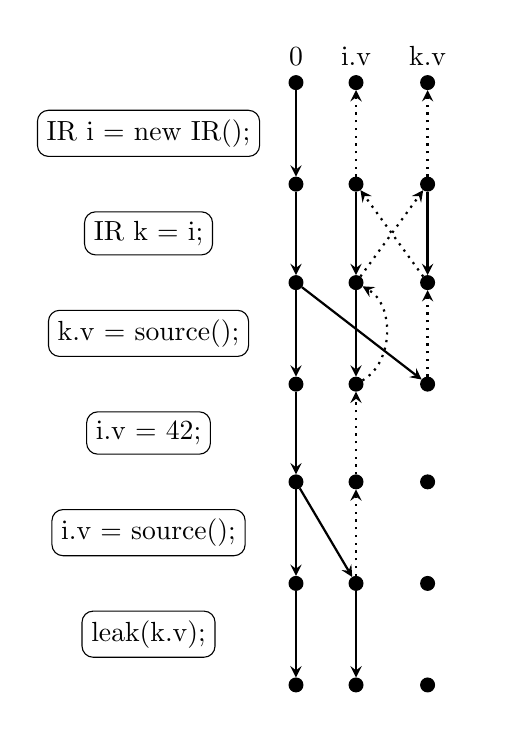
\begin{tikzpicture}[auto,
                s/.style={draw, rounded corners},
                v/.style={draw, fill=black, circle, inner sep=0pt, minimum size=5pt},
                every node/.style={align=center},
                every matrix/.style={ampersand replacement=\&,column sep=0.25cm,row sep=.25cm},
                vto/.style={->, >=stealth, thick},
                ato/.style={->, >=stealth, thick, dotted}]
                \matrix {
                    \& \node[v, label={0}] (zero1) {}; \& \node[v, label={i.v}] (i1) {}; \& \node[v, label={k.v}] (j1) {};\\
                    \node[s] (s1) {\smallcode{IR i = new IR();}}; \& \& \&\\
                    \& \node[v] (zero2) {}; \& \node[v] (i2) {}; \& \node[v] (j2) {};\\
                    \node[s] (s2) {\smallcode{IR k = i;}}; \& \& \&\\
                    \& \node[v] (zero3) {}; \& \node[v] (i3) {}; \& \node[v] (j3) {};\\
                    \node[s] (s3) {\smallcode{k.v = source();}}; \& \& \&\\
                    \& \node[v] (zero4) {}; \& \node[v] (i4) {}; \& \node[v] (j4) {};\\
                    \node[s] (s4) {\smallcode{i.v = 42;}}; \& \& \&\\
                    \& \node[v] (zero5) {}; \& \node[v] (i5) {}; \& \node[v] (j5) {};\\
                    \node[s] (s5) {\smallcode{i.v = source();}}; \& \& \& \&\\
                    \& \node[v] (zero6) {}; \& \node[v] (i6) {}; \& \node[v] (j6) {};\\
                    \node[s] (s6) {\smallcode{leak(k.v);}}; \& \& \& \&\\
                    \& \node[v] (zero7) {}; \& \node[v] (i7) {}; \& \node[v] (j7) {};\\
                };
        
                \draw[vto] (zero1) -- (zero2);
                \draw[vto] (zero2) -- (zero3);
                \draw[vto] (zero3) -- (zero4);
                \draw[vto] (zero4) -- (zero5);
                \draw[vto] (zero5) -- (zero6);
                \draw[vto] (zero6) -- (zero7);
        
                \draw[vto] (zero3) -- (j4);
                \draw[ato] (j4) -- (j3);
                \draw[ato] (j3) -- (i2);
                \draw[ato] (i2) -- (i1);
                \draw[vto] (i2) -- (i3);
                \draw[vto] (i3) -- (i4);
                \draw[vto] (zero5) -- (i6);
                \draw[vto] (i6) -- (i7);
                \draw[ato] (i6) -- (i5);
                \draw[ato] (i5) -- (i4);
                \draw[ato] (i4)[out=30, in=-30] to (i3);
                \draw[ato] (i3) -- (j2);
                \draw[ato] (j2) -- (j1);
                \draw[vto] (j2) -- (j3);
            \end{tikzpicture}
            \caption{Forwards}
            \label{tikz:strongupdate_a}
        \end{subfigure}
        \qquad
        \begin{subfigure}[b]{0.45\textwidth}
            \centering
            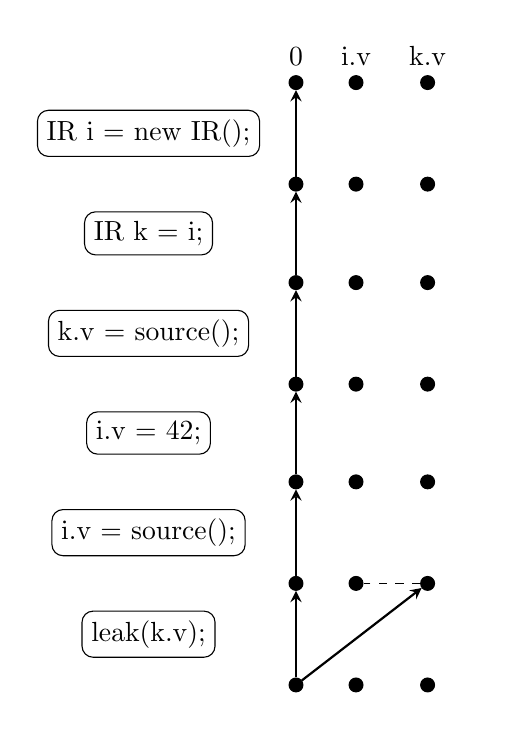
\begin{tikzpicture}[auto, 
                s/.style={draw, rounded corners},
                v/.style={draw, fill=black, circle, inner sep=0pt, minimum size=5pt},
                every node/.style={align=center},
                every matrix/.style={ampersand replacement=\&,column sep=0.25cm,row sep=.25cm},
                vto/.style={->, >=stealth, thick}]
                \matrix {
                    \& \node[v, label={0}] (zero1) {}; \& \node[v, label={i.v}] (i1) {}; \& \node[v, label={k.v}] (j1) {};\\
                    \node[s] (s1) {\smallcode{IR i = new IR();}}; \& \& \&\\
                    \& \node[v] (zero2) {}; \& \node[v] (i2) {}; \& \node[v] (j2) {};\\
                    \node[s] (s2) {\smallcode{IR k = i;}}; \& \& \&\\
                    \& \node[v] (zero3) {}; \& \node[v] (i3) {}; \& \node[v] (j3) {};\\
                    \node[s] (s3) {\smallcode{k.v = source();}}; \& \& \&\\
                    \& \node[v] (zero4) {}; \& \node[v] (i4) {}; \& \node[v] (j4) {};\\
                    \node[s] (s4) {\smallcode{i.v = 42;}}; \& \& \&\\
                    \& \node[v] (zero5) {}; \& \node[v] (i5) {}; \& \node[v] (j5) {};\\
                    \node[s] (s5) {\smallcode{i.v = source();}}; \& \& \& \&\\
                    \& \node[v] (zero6) {}; \& \node[v] (i6) {}; \& \node[v] (j6) {};\\
                    \node[s] (s6) {\smallcode{leak(k.v);}}; \& \& \& \&\\
                    \& \node[v] (zero7) {}; \& \node[v] (i7) {}; \& \node[v] (j7) {};\\
                };
        
                \draw[vto] (zero7) -- (zero6);
                \draw[vto] (zero6) -- (zero5);
                \draw[vto] (zero5) -- (zero4);
                \draw[vto] (zero4) -- (zero3);
                \draw[vto] (zero3) -- (zero2);
                \draw[vto] (zero2) -- (zero1);
        
                \draw[vto] (zero7) -- (j6);
                \draw[dashed] (j6) -- (i6);
            \end{tikzpicture}
            \caption{Backwards}
            \label{tikz:strongupdate_b}  
        \end{subfigure}
        \caption{Strong Update Example}
        \label{tikz:strongupdate}
    \end{figure}

    Searching backwards also allows for easier strong updates. Backwards, the first observed strong update is the last before the sink. 
    
    Consider the example in \autoref{tikz:strongupdate}. \code{IR} is a wrapper around an integer to provide integers by reference. The main idea behind this example is a strong update on an alias of a tainted variable and later retaint the alias. In \ref{tikz:strongupdate_a}, taints are created at both source statements. The critical point is \code{i.v = 42;} where the forwards strong update rule kills \code{k.v} because it must aliases \code{i.v} and the taint \code{i.v}, later found through aliasing, is killed according to normal flow. Both kills are appropriate because it is unknown whether there will be another strong update. This is not the case in backwards analysis. Here the last write before the sink to the leaked variable or one of its aliases is found first. So after one propagation the taint already reaches a source statement.

    \subsection{Backwards Clinit Rule}\label{s:clinitrule}
    \code{<clinit>} is a special method in the JVM and stands for class loader init. The function is generated by the compiler and can not be called explicitly. Examples of statements which get compiled into clinit can be seen in \autoref{lst:clinit_examples}. The invokation is implicit at the initialization phase of the class and is executed at most once for each class \footnote{\url{https://docs.oracle.com/javase/specs/jvms/se8/html/jvms-2.html\#jvms-2.9}}. 
    This behavior is modelled as an overapproximation in \textsc{FlowDroid}'s default call graph algorithm SPARK. SPARK adds an edge to \code{<clinit>} at each statement containing a \code{StaticFieldRef}, \code{StaticInvokeExpr} or \code{NewExpr} \footnote{\url{https://github.com/soot-oss/soot/blob/59931576784b910a7d38f81910b7313aa2feafea/src/main/java/soot/jimple/toolkits/callgraph/OnFlyCallGraphBuilder.java\#L969}}.
   
    \begin{figure}[ht]
        \centering
        \begin{subfigure}[b]{0.45\textwidth}
            \centering
            \begin{lstlisting}[gobble=16]
                class ClinitClass1 {
                    public static string str = source();
                }
            \end{lstlisting}
            \caption{static variable initialization}
            \label{lst:clinit_examples_a}
        \end{subfigure}
        \hfill
        \begin{subfigure}[b]{0.45\textwidth}
            \centering
            \begin{lstlisting}[gobble=16]
                class ClinitClass2 {
                    static {
                        ClinitClass2.sink();
                    }
                }
            \end{lstlisting}
            \caption{static block}
            \label{lst:clinit_examples_b}
        \end{subfigure}
        \caption{Examples of statements being in \code{<clinit>}}
        \label{lst:clinit_examples}
    \end{figure}


    The need for this rule is rooted in the IFDS solver of \textsc{FlowDroid}. The solver decides whether to use normal flow or call flow by calling \code{isCallStmt(Unit u)} on the interprocedural control-flow graph generated by Soot. Internally, this method calls \code{containsInvokeExpr()} on the \code{Unit} object. \code{containsInvokeExpr()} for \code{AssignStmt} only returns true if the right hand side is an instance of \code{InvokeExpr}. Consequently, the calls to \code{<clinit>} from \code{AssignStmt}s with \code{NewExpr} or \code{StaticFieldRef} on the right side are missed.

    The Backwards Clinit Rule manually injects an edge to the \code{<clinit>} method in the infoflow solver when appropriate during the analysis. Also, it lessens the overapproximation of SPARK by carefully choosing whether to inject the edge. The rule works as follows:
    \begin{itemize}
        \item \textbf{Clinit Rule 1}: If the tainted static variable is a field of the methods class: Do not inject because we will at least encounter a \code{NewExpr} of the same class further in the call graph.
        \item \textbf{Clinit Rule 2}: Else if the tainted static variable matches the \code{StaticFieldRef} on the right hand side: Inject the edge because we can not be sure whether we see another edge to \code{<clinit>}.
        \item \textbf{Clinit Rule 3}: Else if the class of the tainted static variable matches the class of the \code{NewExpr}: Inject the edge because we can not be sure whether we see another edge to \code{<clinit>}.
    \end{itemize}
    This is still an overapproximation of course. A precise solution would require bookkeeping of the first occurence in the code of every class. 

    In fowards analysis, the issue is not as severe. As taints are introducted at sources, if the source statement is a static initialization as shown in \autoref{lst:clinit_examples_a}, the propagation starts inside the \code{<clinit>} method. The solver has a \code{followReturnsPastSeeds} option which propagates return flows for unbalanced problems, for example when the taint was introducted inside a method and therefore there was no incoming flow. This allows the forwards analysis to detect leaks originated from static variable initializations but misses leaks inside static blocks as shown in \autoref{lst:clinit_examples_b}.

    \subsection{Other Rules}
    Skip System Class Rule and Stop After First K Flows Rule are not direction-dependent. Both are shared with the forwards search and therefore use the existing implementation in \textsc{FlowDroid}.
    
    % Typing Propagation Rule has no backwards equivalent. We decided to implement type checking in the infoflow problem instead.

    \section{Other Components}
    \subsection{Code Optimizer: AddNOPStmts}
    Before starting the analysis, \textsc{FlowDroid} applies code optimization to the interprocedural call graph. By default, dead code elimination and within constant value propagation is performed. Those are also applied before backwards analysis but we needed another code optimizer to handle an edge case in backwards analysis.

    First, take a look at \code{StatictTestCode#static2Test} in \autoref{lst:static2TestJava}. The method and entry point \code{static2Test} is static and does not have any parameters. Same is true for the source method \code{TelephonyManager#getDeviceId}. Due to the first condition, \code{static2Test} has no identity statements and because of the second  condition there are also no assign statements before the source statement in Jimple. Therefore the source statement is the first statement in the graph. 
    Next, a detail of \textsc{FlowDroid}'s IFDS solver is important. The Return and CallToReturn flow function is only applied if a return site is available \cite{Arzt2017PhD}.
    When searching backwards, the source statement is the last statement and thus has no return sites. Now recall \autoref{s:sourcerule}, taints flowing into sources are registered in the CallToReturn flow function. Altogether, leaks can not be found if the source statement is the first statement.

    Moving the detection of incoming taints flows into sources from the CallToReturn to the Call flow function was not an option because by default source methods are not visited. 
    Our solution is to just add a NOP statement in such cases. This saves us from introducing new edge cases inside the flow functions which are already complex enough. Due to the entry points being known beforehand, the overhead is negligible.

    \begin{figure}[ht]
        \centering
        \begin{subfigure}[b]{\textwidth}
            \begin{lstlisting}[gobble=12]
                public static void static2Test() {
                    String tainted = TelephonyManager.getDeviceId();
                    ClassWithStatic static1 = new ClassWithStatic();
                    static1.setTitle(tainted);
                    ClassWithStatic static2 = new ClassWithStatic();
                    String alsoTainted = static2.getTitle();
                    
                    ConnectionManager cm = new ConnectionManager();
                    cm.publish(alsoTainted);
                }
            \end{lstlisting}
            \caption{Java}
        \end{subfigure}
        \qquad
        \begin{subfigure}[b]{\textwidth}
            \begin{lstlisting}[language=Jimple]
                public static void static2Test() {
                    tainted = staticinvoke <soot.jimple.infoflow.test.android.TelephonyManager: java.lang.String getDeviceId()>(); // Line 2 in (a)

                    // [...]
            
                    virtualinvoke cm.<soot.jimple.infoflow.test.android.ConnectionManager: void publish(java.lang.String)>(alsoTainted); // Line 9 in (a)

                    return;
                }
            \end{lstlisting}
            \caption{Jimple}
        \end{subfigure}
        \caption{static2Test Code}
        \label{lst:static2TestJava}
    \end{figure}

    \subsection{Taint Wrappers}\label{s:taintwrapper}
    \textsc{FlowDroid} already provides an interface \code{IReversibleTaintWrapper} for taint wrappers which also provide inversed summaries. The Summary Taint Wrapper for \textsc{StubDroid} already implements this. For the Easy Taint Wrapper we contributed the inverse implementation.
    
    \subsection{Native Call Handler}
    The native call handler of \textsc{FlowDroid} handles two methods:
    \begin{itemize}
        \item \code{System#arraycopy}: If the first parameter is tainted, taint the second parameter.
        \item \code{reflect.Array#newArray}: If the length is tainted, propagate it over the statement.
    \end{itemize}
    We adapated the existing implementation and only reversed the logic of \code{System#arraycopy} to reflect the analysis direction.

    

\end{document}